% Template for PLoS
% Version 1.0 January 2009
\documentclass[10pt]{article}
%\usepackage[top=0.85in,left=2.75in,footskip=0.75in]{geometry}

% Use Unicode characters when possible
\usepackage[utf8]{inputenc}

% textcomp package and marvosym package for additional characters
\usepackage{textcomp,marvosym}

% fixltx2e package for \textsubscript
\usepackage{fixltx2e}

% amsmath and amssymb packages, useful for mathematical formulas and symbols
\usepackage{amsmath,amssymb}

% cite package, to clean up citations in the main text. Do not remove.
\usepackage{cite}

% Use nameref to cite supporting information files (see Supporting Information section for more info)
\usepackage{nameref,hyperref}

% line numbers
\usepackage[right]{lineno}

% ligatures disabled
\usepackage{microtype}
%\DisableLigatures[f]{encoding = *, family = * }

% Text layout
\topmargin 0.0cm
\oddsidemargin 0.5cm
\evensidemargin 0.5cm
\textwidth 16cm
\textheight 21cm

% Bold the 'Figure #' in the caption and separate it from the title/caption with a period
% Captions will be left justified
\usepackage[aboveskip=1pt,labelfont=bf,labelsep=period,justification=raggedright,singlelinecheck=off]{caption}

% Use the PLoS provided BiBTeX style
\bibliographystyle{plos2015}

% Remove brackets from numbering in List of References
\makeatletter
\renewcommand{\@biblabel}[1]{\quad#1.}
\makeatother

% Leave date blank
\date{}

%% Include all macros below

% graphicx package, useful for including eps and pdf graphics
% include graphics with the command \includegraphics
\usepackage{graphicx}
\usepackage{color}
\usepackage{comment}    % for the supplement org-tbl
\usepackage{placeins}   % for the \FloatBarrier
\usepackage[usenames,dvipsnames,svgnames]{xcolor}          %add color
\usepackage{xspace}                                        %add space at end of macro

%add [disable] to turn all s off
\usepackage[colorinlistoftodos, textsize=footnotesize, linecolor=black!30, backgroundcolor=white]{todonotes}
\usepackage{url}       %for BibTex urls
\usepackage[auth-sc,affil-sl]{authblk} % author: small caps, affiliation: slanted.

\newcommand{\yyy}[1]{\[inline,backgroundcolor=blue!20!white,caption={some comments}]{ #1}}
\newcommand{\etal}{\textit{et al.\ }}
\newcommand{\ordo}{\mathcal{O}}
%% END MACROS SECTION

\title{Comparison of crossover methods for digital genomes of variable length}

\author[1]{Karl Fogelmark}
\author[1]{Adriaan Merlevede}
\author[1]{Carl Troein\footnote{Corresponding author, carl@thep.lu.se}}
\author[1]{Henrik \r{A}hl}
\affil[1]{Computational Biology and Biological Physics, Department of Astronomy and Theoretical Physics, Lund University, 223 62 Lund, Sweden}

\renewcommand\Authands{ and }

\renewcommand{\paragraph}[1]{\textbf{#1}\hspace{2ex}}
\renewcommand{\paragraph}[1]{}

\begin{document}

\maketitle

% http://www.ploscompbiol.org/static/guidelines
% http://www.ploscompbiol.org/static/checklist
% http://www.ploscompbiol.org/static/supportingInformation
% http://www.ploscompbiol.org/static/latexGuidelines
% http://blogs.plos.org/plos/2015/01/streamlined-formatting-plos-article/

%\tableofcontents
%\listofs

% Please keep the abstract below 300 words no abbreviations or citations.
% \section*{Abstract}
\begin{abstract}

% BACKGROUND

\textit{In silico} evolution has applications in computer science and
evolutionary biology. Although most implementations use genomes of constant
length, variable-length genomes are a natural choice when modelling
evolutionary mechanisms such as copy number and structural variations, or
traverse search spaces of variable or unknown dimensionality. However, such
genomes are costly to manipulate and interpret, especially for performing
crossover.

% METHODOLOGY

Here, we compare different crossover methods for variable-length linear
genomes. Qualities used for comparison are the ability of the crossover to
retain homologous features in the parental genomes, CPU time consumption and
performance in a toy evolutionary model.

% PRINCIPAL FINDINGS

We find that existing methods are not fully optimized, neither in terms of
quality of the offspring nor computation time. Crossover
of variable-length genomes is computationally expensive, but
can accelerate evolution when other steps such as fitness evaluation
are also expensive, which is often the case. We show that simple
heuristics can improve the overall performance compared to earlier
methods, and outline directions for further improvements.

\end{abstract}

\newpage


% Please keep the Author Summary between 150 and 200 words
% Use first person. PLOS ONE authors please skip this step.
% no citations allowed
%\section*{Author summary}


\section{Introduction}

% The introduction should put the focus of the manuscript into a broader
% context. As you compose the introduction, think of readers who are not
% experts in this field. Include a brief review of the key literature. If
% there are relevant controversies or disagreements in the field, they
% should be mentioned so that a non-expert reader can delve into these
% issues further. The introduction should conclude with a brief statement of
% the overall aim of the experiments and a comment about whether that aim
% was achieved.

\paragraph{In silico evolution}
Evolutionary experiments are costly and
time-consuming. One alternative way to perform experiments in evolutionary
biology is a computational approach, where instead of biochemical organisms,
instantiations of a virtual model are subjected to iterative reproduction,
mutation and selection. This simulated evolution allows us to study the
general process of evolution, of which life on earth is a special
case.

%While some research has been done in this field, there is moderate skepticism
%in the life sciences community on the relevancy of these in silico experiments
%to life on earth. Indeed, virtual models of evolution cannot hope to approach
%the complexity of biochemical life forms, especially considering our lack of
%knowledge about many aspects of cellular processes. Instead, as is the case in
%all modeling endeavors, models of virtual evolution should strike a balance
%between accuracy and abstraction.

\paragraph{Need for variable-length genomes}
When generalizing results obtained from \textit{in silico} experiments to
biological evolution, or to evolution in general, one has to be mindful of the limitations
and general properties of the model. For example, many existing models use genome
representations with high information density. While computationally efficient
and easily interpretable, it does not leave room for the exploration of neutral
networks, inhibiting neutral evolution and thus changing the evolutionary dynamics
of the system. In addition, in order to investigate the evolution of genome
structure, the model must be rich enough to accommodate insertions and deletions
 as well as concepts such as synteny, modularity, sequence motifs, and
copy numbers.
Linear genomes of variable length do not impose fixed information densities or
structures, and are a natural setting to model genome structure dynamics close
to how it is understood in biology. They can also be of use
in computer science, to traverse search spaces with variable or unknown
dimensionality \cite{lee2000,hutt2007}.
Despite their potential, few past experiments have featured genomes of variable
length, possibly due to their computationally expensive reading and manipulation,
especially when performing crossover.

%In current literature on \textit{in silico} evolution, some researchers have noted the
%lack of focus on model properties such as genome representation and
%genotype-phenotype mapping \cite{gutierrez2014}. Most
%studies attempt to isolate specific properties of interest, in the process
%often abstracting these factors to a high degree, to the point of defining
%mutation and crossover operations on the phenotype directly []. However, some
%qualitative properties of the genotype-phenotype map itself are influential to
%the evolutionary process [], and developing a realistic genome representation
%is especially important when genotypic properties are themselves the topic of
%interest. For example, in order to investigate the evolution of genome
%structure, an accurate model must be rich enough to capture the concepts of
%synteny, modularity, sequence motifs, and copy numbers, and allow these
%features to be mutated and selected. Furthermore, evolving a genetic code with
%very high information density precludes the exploration of neutral networks
%and may inhibit the effects of neutral evolution []. Linear genomes of
%variable length, similar to chromosomes, containing the information for
%multiple metabolical or phenotypical traits (``genes''), are an attractive
%option, but have not been featured in many past experiments. One possible
%explanation is the expensive reading and manipulation of such genomes,
%especially for performing crossover.

\paragraph{Goal of this paper} Herein, we compare existing and new methods for
crossover of variable-length linear genomes consisting of binary digits,
both in an artificial setting of randomly generated
genomes with a given similarity, and in an experimental setting during a toy
evolution. The comparison is based on three properties: the ability of the
crossover to match real homologous sequences, CPU time consumption, and the
success of the algorithm to produce sensible high-fitness offspring (i.e.\ the
number of generations needed to reach a certain fitness level).

%\todo[inline]{The following paragraph makes it sound that our method is bad
%  with current computers, and only in the future might it be relevant}
\paragraph{Application and future prospects}
% Together with ever-increasing computational resources,
We hope that our method, and general approach, can be used in future
research seeking to unravel the mechanisms governing the evolution of
genomic structure and other evolutionary concepts which require variable-length
genome representations. In addition, we hope that it can be of use
in novel approaches to evolutionary computation.

\section{Methods}

\subsection{Crossover algorithms}

Several crossover methods exist for digital genomes of constant size.
In evolutionary algorithms, popular choices include one-point, two-point,
multiple-point and uniform crossover for genomes \cite{yu2010}.
Each algorithm creates two new complementary sequences that together contain all the
sequence information from their parents. Usually, only one of the two  siblings is
retained for selection. Similar strategies
can be used for genomes of variable length, but the added difficulty for
variable-length genomes is to know where to align the crossover points. The
crossover should construct offspring with a high expected fitness by recombining
genomic structures unique to each parent, while keeping the homologous information
present in both.

\paragraph{Hirschberg} One solution is to align the two parental genomes
using a sequence alignment algorithm, prior to choosing the crossover points.
Aligned locations (not including gaps) can then serve as possible sites for crossover
points in the same way as in sequences of constant length. Because the
appropriate number of crossover points should increase with genome length,
it is natural to give each aligned bit the same probability of acting as a
crossover point. Many alignment methods exist (for review, see \cite{haque2009}).
Because it is simple and theoretically well-founded, we chose to use the Hirschberg
algorithm with an affine gap penalty as described by Myers and
Miller~\cite{hirschberg1975,myers1988}. This is an adaptation of the traditional Needleman-Wunsch that lowers
the memory complexity from $\ordo{}(N^2)$ to $\ordo{}(N)$ while retaining the
$\ordo{}(N^2)$ time complexity. Our implementation
uses a binary alphabet, where alignments are scored $+1$ for a match, $-5$
for a mismatch, and an affine gap penalty of $-20$ to open and $-3$ to
extend. These numbers, though largely arbitrary, were selected to produce
results in agreement with a manual alignment.
%\todo{what does Hirchberg use/recommend? Does different number have some impact/significance in one way or the other?}
%\todo{example: insertion/deletion preferred if about 13 bits apart - but we're not actually considering max likelihood.}

\paragraph{Heuristic} To lower the time consumption of the alignment process
for crossover, we implemented a simple heuristic method for quickly breaking down the
alignment problem, under the assumption that the parental genomes are usually
highly similar. This recursive heuristic algorithm extracts three substrings of
length 64~bits, centred at one, two and three quarters of one of the genomes. For each
of these three subsequences, the other genome is scanned for matching regions with
a Hamming distance $\le 20$. If at least two of the three yield a well-defined
best match (lowest Hamming distance), and if
the matches occur in the correct order without overlap, the two genomes are
cut in the corresponding positions and the pieces are aligned by recursion. If
these conditions are not met, or if the genomes are shorter than 256~bits, the
method falls back on the Hirschberg algorithm.

\paragraph{Synapsing} An alternative method was proposed by Hutt and Warwick,
inspired by the chi structure of chromosomes during meiosis in biology
\cite{hutt2007}. Their synapsing method finds and aligns the longest common
subsequence of the two parental genomes (a synapse). This is recursively
repeated on the left and right sides of the synapse, until no longest common
subsequence above a specified threshold length can be found. This results in an
alternating pattern of synapses, where both parental genomes are identical, and
unaligned regions, where they are not. The bits contained in synapses are used
as possible crossover points in a
multi-point crossover, exchanging the unaligned regions in between.
In our implementation, the minimum synapse length was set to 3 bits.
For both the synapsing crossover and the alignment-based methods,
each aligned bit had a probability of $0.02$ to serve as a
crossover point.

%\paragraph{Aligned synapsing}
%In order to compare the Hirschberg and synapsing crossover methods, we chose
%to implement the synapsing crossover as an alignment algorithm. The synapsed
%parts are seen as matches between the two parental sequences, while the
%remaining gaps are seen as insertions and deletions. Because the synapsing
%method does not distinguish between gaps and mismatches, we also consider an
%alternative alignment representation where non-synapsed regions of the same
%length and shorter than 21 bits are considered mismatches rather than gaps.

\subsection{Benchmark evolution}
Ultimately, what defines a good crossover is its ability to produce
high-fitness offspring and accelerate evolution. While the
potential of any crossover to do so
 is strongly dependent on the genome structure, we chose to compare
the evolutionary dynamics resulting from different crossover methods in a
toy evolution model that we think is representative of many interesting
and useful situations. Similar models have been used in literature
(e.g., \cite{batut2013,beslon2010}).
The genomes and their relation to the phenotype and evolution target are
structured enough to allow crossover to combine useful building blocks of
both parents' genomes, and complex enough to present a complex dynamical
genomic structure \cite{batut2013}.

\paragraph{Geno- and phenotypes} In the model, we choose to represent each
individual's phenotype as a function $f:
[0,1]\rightarrow \mathbb{R}$, described by a sum of
triangular basis functions. Each gene in the genome codes for an isosceles
triangle of height $h\in[-1,1]$ and base $b\in(0,1]$, which rests on the $x$
axis centred at a point $s\in[0,1]$. A gene is defined by a start sequence
(110011), followed by three sets of ten bits each for the
parameters $h$, $b$ and $s$. These are encoded as binary integers which are then
rescaled to the relevant ranges. A gene can be recognized
anywhere in the genome, except inside another gene. The phenotype is
calculated by summing the triangles represented by all genes. The
fitness function, $F$, is defined by the distance of the phenotype to the target
function $g(x) = \sin(6\cdot 2\pi x)$, measured as the $L^2$ norm,
$F = -\int_0^1{(f(x)-g(x))^2}dx$.

\paragraph{What about the sign of the fitness? In the above it is positive.
Call it a cost and change fig 3?}

\paragraph{Selection method}
Selection is effected by a tournament method. In each generation, two random
individuals are chosen, and the one with the lowest fitness is removed from
the population. It is replaced by a new individual generated either
through crossover (with probability $p_X$) or mutation (with probability $1-p_X$).
In either case, parents are picked by taking the individual with the highest
fitness from a random sample of two. For crossover, the two parents must be
distinct.

\paragraph{Mutation} In the case of mutation, one of three operators is
executed: substitution (probability 0.8), deletion (probability 0.1), or
insertion (probability 0.1). During substitution, each bit in the genome is
flipped with probability 0.001. During deletion or insertion, a random
sequence section of random length $l$, drawn from a power law distribution
proportional to $l^{-2}$ (not longer than the length of the genome), is
removed from the sequence or is repeated in a random genomic location. A
similar power law distribution for the size of insertions and deletions has
been observed in nature~\cite{cartwright2009}.

\section{Results}

\paragraph{Preservation of homology} As an initial comparison, we view each
crossover method as a sequence alignment. Figure~\ref{fig:align}A-B shows the
alignment score thus obtained. By design, the Hirschberg method gives the globally
optimal value. Our heuristic algorithm also performs optimally, unless the two parents are
highly divergent; thus the heuristic is highly similar to the
Hirschberg method in most cases. However, the alignment score is not a good measure
of success for crossover. Aside from being arbitrary, it is a poor proxy for the evolutionary
history of divergent sequences, and it does not measure the properties of the resulting offspring.
Specifically, the synapsing method is not optimized as an alignment algorithm and produces
an excessive number of small gaps, resulting in low alignment scores.

In order to better compare the ability of the crossovers to propagate
genetic information shared by the two parents, we measured the fraction of homologous
bits that were consistently inherited after crossover.
More precisely, for each method, we performed a large set of crossovers,
each resulting in a pair of complementary offspring. In each case, one of the
parents was a copy of the other, mutated to some degree. With the exception of
bits involved in insertion or deletion, each bit in either parental genome can be
matched uniquely to an unchanged or substituted bit in the other, resulting in
a set of homologous bit pairs. Here, homology is used in the biological sense,
i.e.\ sequence features that are shared because they descend from the same ancestral
original.\footnote{In our system, insertions can also result in paralogy, i.e.\ sequences that share a common history
through duplication inside the same genome. This kind of homology is not considered here.}
Figure~\ref{fig:align}C-D shows
the fraction of such homologous pairs that were divided evenly among the two
complementary offspring. That is, both homologous offspring should have exactly
one of the two homologous bits.

All methods preserve a large fraction of the existing homology when the parental
sequences are similar. In general, the Hirschberg method outperforms the other
two methods in this regard. The heuristic method performs similarly unless the parents are highly dissimilar;
in particular, insertions of duplicated genetic material will increase the risk
of misidentifying the cutting points for the heuristic algorithm.
For dissimilar sequences, the synapsing method preserves much less homology than
the alignment-based methods.
It should be noted that $10\%$ sequence divergence is high and unlikely to occur
often during most evolutionary experiments; in nature, organisms with such
dissimilarity are unlikely to produce fertile offspring.

\paragraph{CPU time consumption} To assess the performance of these methods in
practical computation, we compared their CPU usage. Figure~\ref{fig:time} shows
CPU cost as a function of genome length and sequence dissimilarity. The heuristic
and synapsing methods are much faster than Hirschberg, which has quadratic
complexity.
%As before, the heuristic gives a good approximation of Hirschberg but is
%sensitive to insertions and deletions.
The computational cost of the Hirschberg and synapsing alignment methods do not
depend strongly on the similarity between the parental sequences. In contrast,
the heuristic method is fast for similar genomes, but breaks down when the parents are
highly dissimilar, as it increasingly falls back on the Hirschberg method.
For most applications, sequence divergence is usually low and the heuristic method
is approximately twice as fast as the synapsing method.

\paragraph{Evolutionary success} Finally, we compared the ability of the
crossovers to perform successful sexual reproduction in a model evolutionary
experiment. Figure~\ref{fig:cost}A shows the progression of the increasing fitness of
the population over time. The results of the heuristic alignment and synapsing methods
are similar. Note that, in this experiment, evolution is faster with crossover than
without. Figure~\ref{fig:cost}B gives the speed of evolution
for different crossover probabilities. Again, the two methods perform similarly,
with the convergence time minimized around $p_X=0.3$. However, faster convergence
in number of generations is offset by the computational cost of the crossover (Figure~\ref{fig:cost}C).
In our simple benchmark evolution, most calculations are trivial and crossover is
the most time-consuming step. In contrast, most applications have complex fitness functions
that are often much more costly to compute.
In that case, faster convergence speed in number of generation means fewer
fitness evaluations and lower computational cost overall. This is
illustrated in Figure~\ref{fig:cost}D, where the heuristic alignment
method is the fastest by a narrow margin.

\begin{figure}[p]
  \centering
  \includegraphics[width=\textwidth]{figures/fig_alignscore.eps}
  \caption{\textbf{Comparison of alignments and crossovers.}
    (A-B) The quality of alignment between a random genome of length $5000$ bits
    and a mutated version thereof, for global alignment with the Hirschberg
    method (red squares) and the heuristic described in the text
    (black circles). For comparison, the synapsing method is also included,
    treating unsynapsed regions as gaps (blue triangles), or as aligned (with
    mismatches) when they are the same length and shorter than 21 bits (green diamonds).
    (C-D) The fraction of homologous pairs of bits in the parent genomes
    that are present in both offspring genomes, for various levels of sequence
    dissimilarity between the parents.
    The methods were examined using only point mutations (A,~C) or a 40:1:1
    mix of point mutations, insertions and deletions (B,~D). Sequence
    divergence here measures the fraction of bits affected by mutation. Data
    from 400 genomes and mutated partners, each crossed over 100 times (in C-D).
    % The alignment is done 400 times, the crossover more because it's so
    % cheap in comparison.
    Error bars indicate the standard error of the mean.
    %
  }
  \label{fig:align}
\end{figure}

\begin{figure}[p]
  \centering
  \includegraphics[width=\textwidth]{figures/fig_time.eps}
  \caption{\textbf{Run time of genome alignment.}
    (A-B) The time required to align two genomes of given length for crossover
    using the
    Hirschberg method (red squares), the heuristic alignment method (black circles) and
    the synapsing crossover method (blue triangles) on an Intel Core i7 processor.
    The two genomes were separated by point mutations affecting $5\%$ of the
    bits. $\mathcal{O}(N^2)$ and $\mathcal{O}(N \ln N)$ scaling is indicated
    by short and long dashed gray lines, respectively.
    (C-D) The relationship between sequence similarity and the required CPU
    time for the different crossover methods. The sequence divergence
    between the two parental genomes is defined as the fraction of bits affected
    by mutation. The mutations used were only point mutations (A,~C) or a
    40:1:1 mixture of point mutations, insertions and deletions (B,~D).
    Error bars indicate the standard error of the mean.
    %
  }
  \label{fig:time}
\end{figure}

\begin{figure}[p]
  \centering
  \includegraphics[width=\textwidth]{figures/fig_cost.eps}
  \caption{\textbf{The effect of crossover in optimization.}
    (A) Fitness of the best individual in each generation, using the
    heuristic alignment crossover method (solid line) or synapsing crossover
    (blue points) with crossover probability $p_X=0.3$,
    compared with evolution without crossovers (dashed line).
%    The Hirschberg method
%    is not shown because all datapoints overlap with the heuristic. % No, just too slow.
%    The two crossover methods perform similarly
%    and result in faster evolution than without crossover  % Too results-y IMHO.
    (B) The number of generations needed to reach a high fitness ($F=-30$), as a
    function of the crossover probability, $p_X$, for the heuristic alignment method
    (black circles) and synapsing crossover (blue triangles). The Hirschberg method
    was excluded due to its computational cost. For this specific system, the optimal
    crossover rate for optimization is around $p_X=0.3$.
    (C) The amount of CPU time needed to reach fitness $F = -30$ on an
    Intel Core i7 processor. Despite lowering the number of generations needed,
    crossover increases the total required CPU time.
    (D) The same as (C), for a hypothetical experiment where the computational
    cost of fitness evaluation is drastically increased from 0.1 to 15~msec per
    evaluation.
    In this case, the optimal crossover rate is a compromise between the cost of
    crossovers and the decreased number of generations needed to reach the
    target fitness.
  }
  \label{fig:cost}
\end{figure}

\section{Discussion}
From these results, we conclude that alignment-based methods are a good basis
for creating crossover algorithms. The Hirschberg alignment produces high-quality
offspring that retain the homologous features present in both parents, while also recombining
unique features.

Synapsing is outperformed in several ways by the alignment-based methods. The results
from Figure~\ref{fig:align} suggest that synapsing is much less likely to retain the
original properties of the parental genomes. In our benchmark evolution experiment,
synapsing is also slower than the heuristic method. One potential problem
with synapsing is that it only considers local comparisons between the two parental
genomes, not the greater context. As the number of mutations separating the two
genomes grows, the longest common subsequence is shortened and there is an increased
risk of synapsing two unrelated parts. However, different crossover can also confer different
qualitative behaviour on the evolutionary dynamics, other than simply influencing the speed,
which may be useful or interesting in some contexts.
For example, the inability of the synapsing crossover to retain shared homologous sequences
from both parents when they are dissimilar may result in a spontaneous similarity
selection, reproductive isolation, or genomic restructuring events.

Both approaches leave a lot of room for improvement. The quick and dirty
heuristic presented here has a significantly lower computation time than the Hirschberg
method, at low cost in performance. It is likely that other heuristics can further
improve on alignment-based crossover. For the synapsing method, we expect that it can be
improved by using a less rigid and faster local alignment algorithm to find
suitable synapses, rather than the longest common subsequence.

% CONCLUSIONS/SIGNIFICANCE
In the future, we believe that research in new types of evolutionary dynamics and
new genome representations, together with the continued increase in computation power,
will make more complex \textit{in silico} evolution possible. Such
experiments may use our findings to select or develop a suitable
crossover algorithm.


%\section*{Acknowledgments}
%We thank the flying spaghetti monster.

% \nolinenumbers xxx

\section*{Author Contributions}
CT and HÅ conceived the heuristic alignment method.
CT, AM and KF designed the study.
KF, AM, HÅ and CT wrote the computer programs.
AM and CT wrote the manuscript with input from KF and HÅ.
KF and CT prepared the figures.

\subsection*{Funding}
AM, CT and KF were supported by grant 621-2010-5219 from the Swedish Research
Council, \url{http://vr.se/}.

%\section*{Supporting information}
%
%\renewcommand\thefigure{S\arabic{figure}}
%%\renewcommand{\figurename}{Text}
%\setcounter{figure}{0}

%\subsection*{S1 Data}
%\label{S1_data}
%{\bf Data.} This includes all data generated from the analysis of the networks.


%\section*{References} xxx
% Either type in your references using
% \begin{thebibliography}{}
% \bibitem{}
% Text
% \end{thebibliography}
%
% OR
%
% Compile your BiBTeX database using our plos2015.bst
% style file and paste the contents of your .bbl file
% here.

\bibliography{manus}

\end{document}
